%% LyX 2.3.6.1 created this file.  For more info, see http://www.lyx.org/.
%% Do not edit unless you really know what you are doing.
\documentclass[english]{article}
\usepackage[T1]{fontenc}
\usepackage[latin9]{inputenc}
\usepackage{float}
\usepackage{amsmath}
\usepackage{cancel}
\usepackage{graphicx}

\makeatletter

%%%%%%%%%%%%%%%%%%%%%%%%%%%%%% LyX specific LaTeX commands.
%% A simple dot to overcome graphicx limitations
\newcommand{\lyxdot}{.}


\makeatother

\usepackage{babel}
\begin{document}
\begin{figure}[H]
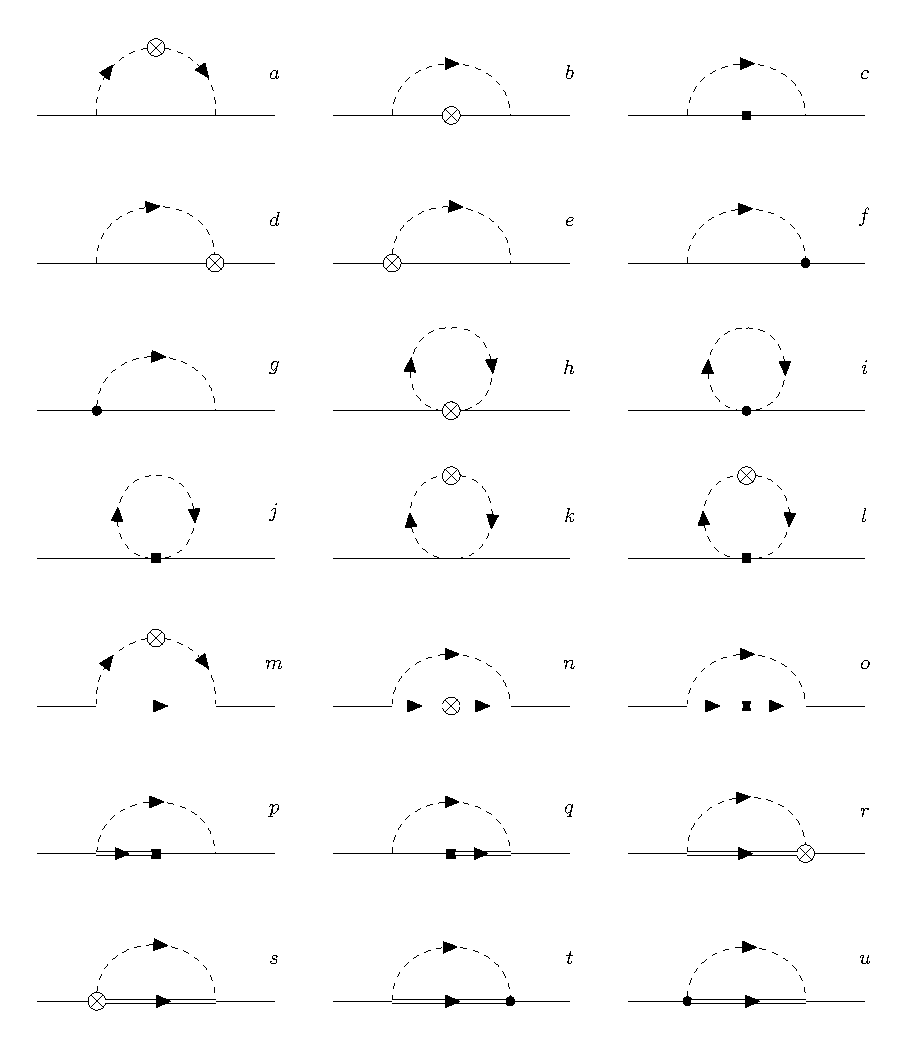
\includegraphics{23411/fig1}

\caption{the one loop Feynman diagrams}
\end{figure}


\part{tadpole}

\section{diagram i}

For the diagram i, the amplitude is 

\begin{align*}
\Gamma_{i}^{+} & =\bar{u}(p')\frac{C_{\phi\phi}}{f^{2}}\int\frac{d^{4}k}{(2\pi)^{4}}\tilde{F}(k)\frac{i}{D_{\phi}(k)}2\cancel{k}\frac{(2k+q)^{+}}{2kq+q^{2}}[\tilde{F}(k+q)-\tilde{F}(k)]\delta(y+\xi-\frac{k^{+}}{P^{+}})u(p)\\
 & =\bar{u}(p')[\gamma^{+}f+\frac{\sigma^{+\nu}q_{\nu}}{2M}g]u(p)
\end{align*}

To get the splitting function we need to calculate these two trace
\begin{align*}
A & =\textrm{Tr}[\Gamma_{i}^{+}(\cancel{p}+M_{N})\gamma^{+}(\cancel{p'}+M_{N})]\\
 & =\frac{C_{\phi\phi}}{f^{2}}\int\frac{d^{4}k}{(2\pi)^{4}}\textrm{Tr}[2\cancel{k}\frac{(2k+q)^{+}}{2kq+q^{2}}(\cancel{p}+M_{N})\gamma^{+}(\cancel{p'}+M_{N})]\tilde{F}(k)\frac{i}{D_{\phi}(k)}[\tilde{F}(k+q)-\tilde{F}(k)]\delta(y+\xi-\frac{k^{+}}{P^{+}})\\
 & =\int\frac{d^{4}k}{(2\pi)^{4}}(\frac{a_{1}}{D_{\phi}(k)D_{\Lambda}^{4}(k)D_{\Lambda}^{2}(k+q)}+\frac{a_{2}}{D_{\phi}(k)D_{\Lambda}^{4}(k)})\delta(y+\xi-\frac{k^{+}}{P^{+}})
\end{align*}
 
\begin{align*}
B & =\textrm{Tr}[\Gamma_{i}^{+}(\cancel{p}+M_{N})(\cancel{p'}+M_{N})]\frac{P^{+}}{M}\\
 & =\frac{C_{\phi\phi}}{f^{2}}\int\frac{d^{4}k}{(2\pi)^{4}}\textrm{Tr}[2\cancel{k}\frac{(2k+q)^{+}}{2kq+q^{2}}(\cancel{p}+M_{N})(\cancel{p'}+M_{N})]\frac{P^{+}}{M}\tilde{F}(k)\frac{i}{D_{\phi}(k)}[\tilde{F}(k+q)-\tilde{F}(k)]\delta(y+\xi-\frac{k^{+}}{P^{+}})\\
 & =\int\frac{d^{4}k}{(2\pi)^{4}}(\frac{b_{1}}{D_{\phi}(k)D_{\Lambda}^{4}(k)D_{\Lambda}^{2}(k+q)}+\frac{b_{2}}{D_{\phi}(k)D_{\Lambda}^{4}(k)})\delta(y+\xi-\frac{k^{+}}{P^{+}})
\end{align*}

where 
\[
\tilde{F}(k)=(\frac{\Lambda^{2}-m_{\phi}^{2}}{D_{\Lambda}(k)})^{2}\,D_{\Lambda}(k)=\Lambda^{2}-k^{2}
\]

If the power of the $k^{-}$ in the denominator of the integral and
the $k^{-}$ in the numerator are same when $k^{+}$ is 0 , the integral
should contain a $\delta$ term. In this case, the power of $k^{-}$
in denominator and numerator are both 2. In the previous paper, we
have some equations to calculate the $\delta$ term, one them is 
\[
\int\frac{d^{4}k}{(2\pi)^{4}}\frac{1}{D_{\phi}(k)D_{\Lambda}^{4}(k)}\delta(y+\xi-\frac{k^{+}}{P^{+}})=\int d^{2}k^{\perp}\int dx\frac{\Gamma(5)}{\Gamma(1)\Gamma(4)}\frac{1}{4!}x(1-x)^{4}\frac{\partial^{3}}{\partial^{3}\Omega}\frac{2\pi i}{k^{\perp2}+\Omega}\delta(y+\xi)
\]

So I separate the numerator of the integral in this form. First, $\textrm{numerator of }A$
can be expressed as 
\[
\textrm{numerator of }A=c_{1}(k^{-})^{2}+c_{2}k^{-}+c_{3}
\]

where $c_{i}$ represent the coefficient. Then I put the $c_{1}(k^{-})^{2}$
in this term $D_{\Lambda}^{2}(k+q)*a_{2}$ which means 
\begin{align*}
\textrm{numerator of }A & =a_{1}+D_{\Lambda}^{2}(k+q)*a_{2}\\
a_{2} & =\frac{c_{1}}{((k^{+})^{2}+2k^{+}q^{+}+(q^{+})^{2})}\\
D_{\Lambda}^{2}(k+q) & =(\Lambda^{2}-(k+q)^{2})^{2}\\
 & =((k^{+})^{2}+2k^{+}q^{+}+(q^{+})^{2})(k^{-})^{2}+...
\end{align*}

With this transition, the power of $k^{-}$ in $a_{1}$ is 1 when
$k^{+}$is 0 which means the $a_{1}$ term does not contain $\delta$
term and the $a_{2}$ is the $\delta$ term and can be calculated
using the equation.The $a_{1}$ and $a_{2}$ in diagram i is given
as
\begin{align*}
a_{1} & =2(2k^{+}+q^{+})^{2}(m_{\phi}^{2}-\Lambda^{2})^{4}\\
 & (\frac{(2k^{+}+q^{+})((k^{\perp}+q^{\perp})^{2}-k^{-}q^{+}-q^{+}q^{-}-k^{+}(k^{-}+q^{-})+\Lambda^{2})^{2}(-2P^{+}q^{+}+q^{+2}-4P^{+2}(1+\xi))}{(k^{+}+q^{+})^{2}}\\
 & +(k^{\perp2}+(k^{\perp}+q^{\perp})^{2}-2k^{+}k^{-}-k^{-}q^{+}-k^{+}q^{-}-q^{+}q^{-}+2\Lambda^{2})\\
 & *(2(k^{\perp}+q^{\perp})^{2}P^{+}-4(p^{\perp}-k^{\perp})^{2}P^{+}-4M_{N}^{2}P^{+}-4k^{-}P^{+2}\\
 & -4k^{+}P^{+}P^{-}+4P^{+2}P^{-}-(k^{\perp}+q^{\perp})^{2}q^{+}-2k^{-}P^{+}q^{+}+k^{-}q^{+2}\\
 & +k^{\perp2}(2P^{+}+q^{+})-2k^{+}P^{+}q^{-}+k^{+}q^{+}q^{-}-2P^{+}q^{+}q^{-}+q^{+2}q^{-}\\
 & -4k^{-}P^{+2}\xi+4P^{+2}P^{-}\xi-(2k^{+}-2P^{+}+q^{+})q^{2})\\
a_{2} & =\frac{2(2k^{+}+q^{+})^{2}(m_{\phi}^{2}-\Lambda^{2})^{4}}{(k^{+}+q^{+})^{2}}(2P^{+}q^{+}-q^{+2}+4P^{+2}(1+\xi))
\end{align*}
 

Then we can get the normal and $\delta$ term of $f$ and $g$

\begin{align*}
f & =f_{res}+\delta f\\
g & =g_{res}+\delta g
\end{align*}

The $g$ is 0 for diagram i. The $f_{res}$ is showed in fig.2. And
the $\delta$ term, $\delta f=-0.0977421\delta(y+\xi)$. The result
of $f$ and $g$ can be checked by compare the integral with the previous
form factor work.
\begin{equation}
F_{1}=\widetilde{F}(q)\int dy(f_{res}+\delta f)
\end{equation}

where $\widetilde{F}(q)$ is the regulator of photon which we introduce
by hand in form factor calculation to get the $Q^{2}$ dependence.
In GPD calculation this $Q$ dependence comes from the input GPD.
The result of eq.1,with $Q^{2}=1$ is $0.0324215*\widetilde{F}(1)=0.00810537$,
while the result in form factor is $0.00810465$

\begin{figure}
\includegraphics[scale=0.5]{424/fres-xi0\lyxdot 1}

\caption{$f_{res}$($\xi=0.1,Q^{2}=1GeV^{2}$) }

\end{figure}

The positive part of $f_{res}$ is small but not zero which is showed
in Fig.3. To check whether the $f_{res}$ is $\delta$ function when
$\xi$ is 0, I have these $\xi f_{res}$ figure showed in Fig.4.

\begin{figure}
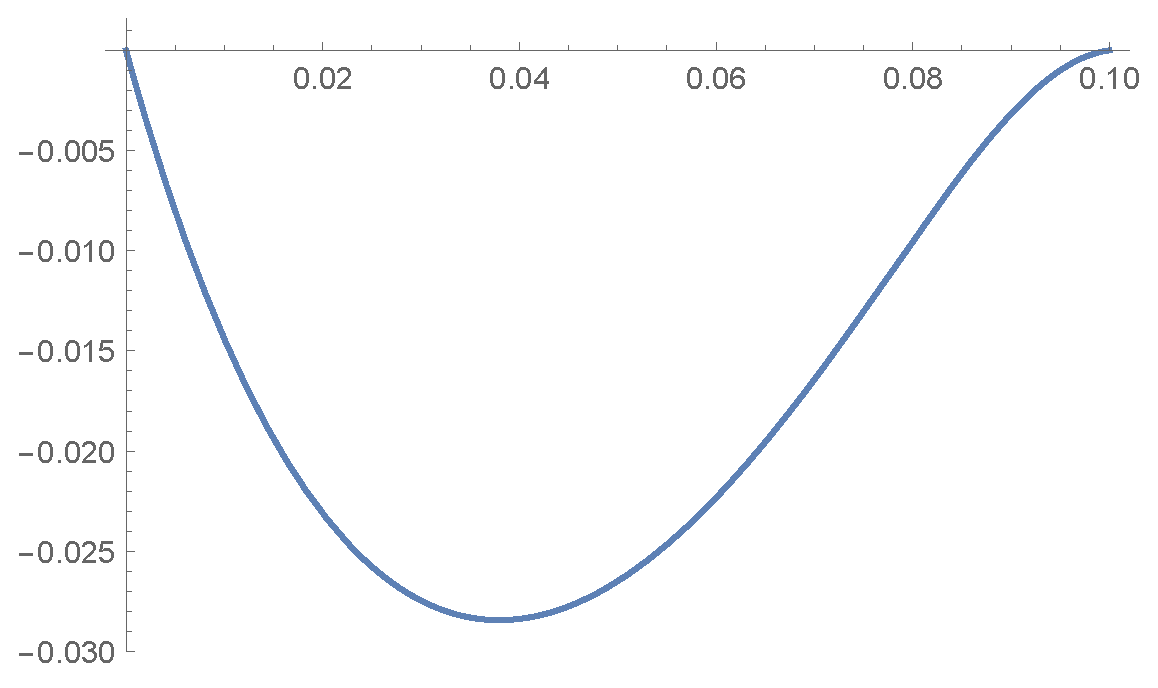
\includegraphics[scale=0.5]{424/fres-zheng}\caption{$f_{res}(y),y>0$}

\end{figure}

\begin{figure}
\includegraphics[scale=0.5]{424/xi-fres-delta}

\caption{$\xi f_{res}$ with $\xi=0.1,0.01,0.001,0.0001$}
\end{figure}

Still the positive part is not zero and is showed in Fig.5. And these
two figure prove that $f_{res}$ approach to the $\delta(y+\text{\ensuremath{\xi}})$
in the zero skewness. 

\begin{figure}
\includegraphics[scale=0.5]{424/xi-fres-zheng}

\caption{$\xi f_{res}(y),y>0$ }

\end{figure}

\begin{figure}
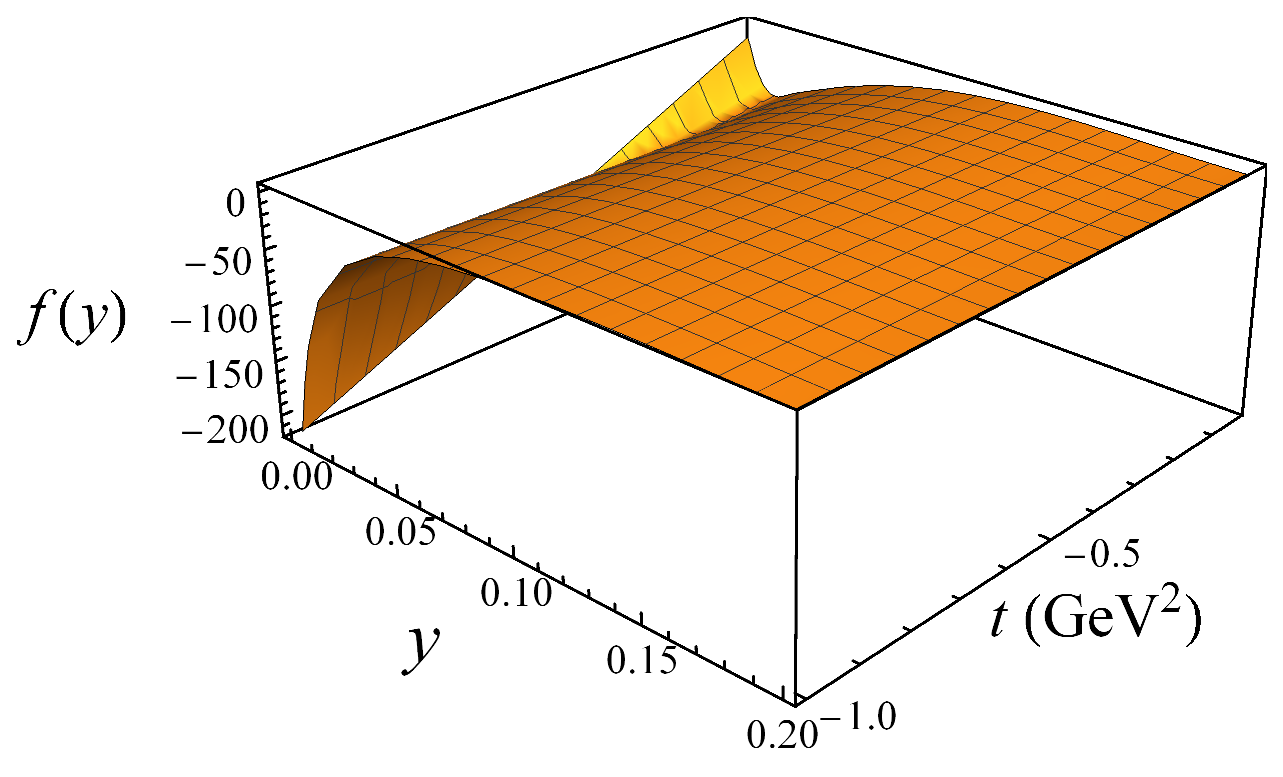
\includegraphics[scale=0.5]{pic/i-f-3D}

\caption{3 dimension picture from diagram i}
\end{figure}


\part{Octet}

\section{diagram b and c (rainbow)}

For diagram b in Fig1, the contribution is 
\[
\Gamma_{b}^{+}=\int\cancel{k}\gamma_{5}\widetilde{F}^{2}(k)\frac{1}{D_{\phi}(k)}\frac{\cancel{p'}-\cancel{k}+m_{N}}{D_{B}(p'-k)}\gamma^{+}\frac{\cancel{p}-\cancel{k}+m_{N}}{D_{B}(p-k)}\cancel{k}\gamma_{5}\delta(y-\frac{k^{+}}{P^{+}})
\]

I do the same separate in diagram i case. The $A$ part is 
\begin{align*}
A_{b} & =\text{\ensuremath{\int(\Lambda^{2}-m_{\phi}^{2})^{4}\frac{\textrm{Tr}[\cancel{k}\gamma_{5}(\cancel{p'}-\cancel{k}+m_{N})\gamma^{+}(\cancel{p}-\cancel{k}+m_{N})\cancel{k}\gamma_{5}]}{D_{\Lambda}^{4}(k)D_{\phi}(k)D_{B}(p'-k)D_{B}(p-k)}}}\delta(y-\frac{k^{+}}{P^{+}})\\
 & =\int\frac{d^{4}k}{(2\pi)^{4}}(\frac{b_{1}}{D_{\Lambda}^{4}(k)D_{\phi}(k)D_{B}(p'-k)D_{B}(p-k)}+\frac{b_{2}}{D_{\phi}(k)D_{\Lambda}^{4}(k)})\delta(y-\frac{k^{+}}{P^{+}})
\end{align*}

Then first term is normal integral which can be calculated with residue
theorem and the second term is $\delta$ term. The normal part can
be expressed as 
\begin{multline*}
\int\frac{d^{4}k}{(2\pi)^{4}}\frac{b_{1}}{D_{\Lambda}^{4}(k)D_{\phi}(k)D_{B}(p'-k)D_{B}(p-k)}\delta(y-\frac{k^{+}}{P^{+}})\\
=\int\frac{d^{4}k}{(2\pi)^{4}}(\frac{b'_{1}k^{-}}{D_{\Lambda}^{4}(k)D_{\phi}(k)D_{B}(p'-k)D_{B}(p-k)}+\frac{b_{1}''}{D_{\Lambda}^{4}(k)D_{\phi}(k)D_{B}(p'-k)D_{B}(p-k)})\delta(y-\frac{k^{+}}{P^{+}})
\end{multline*}

This week, I check the integral above. The integral should have no
issue and the contribution of diagram b can be calculated using the
similar method as diagram i. Last week I made a mistake in my program.
The splitting function can be expressed as
\begin{align*}
f & =f_{1}+f_{2}+f_{\delta}\delta(y)\\
g & =g_{1}+g_{2}+g_{\delta}\delta(y)
\end{align*}

the $f_{1}+f_{2}$ means the normal part of the splitting function
which is separated in $k^{+}=(1-\xi)P^{+}$ due to the singularity
comes from $D_{B}(p'-k)=(p'-k)^{2}-M^{2}+i\epsilon$ change it's position
from upside to the down side of the axis and the $f_{\delta}\delta(y+\xi)$
is the $\delta$ term. 

The splitting function should satisfy that $\int_{-\xi}^{1}dyf(y)$
and $\int_{-\xi}^{1}dyg(y)$ are $\xi$ independent. For diagram b,
the result is, with $\xi=0.1,0.2$, ignore some coefficient
\[
\int_{-\xi}^{1-2\xi}dyf_{1}(y)+\int_{1-2\xi}^{1}dyf_{2}(y)+f_{\delta}=7.27795
\]

and 
\[
\int_{-\xi}^{1-2\xi}dyg_{1}(y)+\int_{1-2\xi}^{1}dyg_{2}(y)+g_{\delta}=-6.566548599
\]

When $\xi=0.1,Q^{2}=1GeV^{2}$, the splitting function looks like
this 
\begin{figure}
\includegraphics{pic/b-f1}

\caption{$f_{1}$from diagram b}

\end{figure}

\begin{figure}
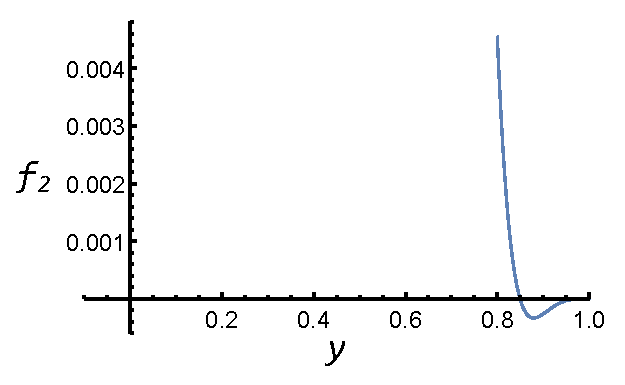
\includegraphics{pic/b-f2}

\caption{$f_{2}$from diagram b}

\end{figure}

\begin{figure}
\includegraphics{pic/b-g1}

\caption{$g_{1}$from diagram b}
\end{figure}

\begin{figure}
\includegraphics{pic/b-g2}

\caption{$g_{2}$from diagram b}
\end{figure}

The $\delta$ term is 
\begin{align*}
f_{\delta}\delta(y+\xi) & =5.2702\delta(y+\xi)\\
g_{\delta}\delta(y+\xi) & =0
\end{align*}

As to zero skewness case, the diagram b in fig.1 is different from
previous diagram. In previous calculation including the tadpole and
meson loop contribution, the reason why the normal integral turns
to a $\delta$ function when $\xi$ goes to zero is the denominator
of these integral. For example, in the tadpole diagram, the normal
integral can be expressed as
\begin{equation}
\int d^{4}k\frac{c_{1}k^{-}+c_{2}}{D_{\phi}(k)D_{\Lambda}^{4}(k)D_{\Lambda}^{2}(k+q)}
\end{equation}

When $\xi=0$, the first two term of denominator of eq.2 have no changes.
The last term $D_{\Lambda}^{2}(k+q)$ will become, notice that $\xi=0$
means $q^{+}=0$ 
\begin{align*}
D_{\Lambda}^{2}(k+q) & =(k^{+}+q^{+})(k^{-}+q^{-})-(k^{\perp}-q^{\perp})^{2}-\Lambda^{2}+i\epsilon\\
 & =k^{+}(k^{-}+q^{-})-(k^{\perp}-q^{\perp})^{2}-\Lambda^{2}+i\epsilon
\end{align*}

Then if we choose $k^{+}=0$, the denominator of integral does not
have the $k^{-}$ and the integral will become like 
\[
\int dk^{-}\frac{c_{1}k^{-}+c_{2}}{D_{\phi}(k)D_{\Lambda}^{4}(k)D_{\Lambda}^{2}(k+q)}=\int k^{-}(c'_{1}k^{-}+c'_{2})
\]

This is a line divergence. And when $k^{+}\neq0$, the imaginary part
of singularities of the integral are same
\begin{align*}
k^{-} & =\frac{-i\epsilon}{k^{+}}+\frac{(k^{\perp}-q^{\perp})^{2}+\Lambda^{2}}{k^{+}}-q^{-}\\
k^{-} & =\frac{-i\epsilon}{k^{+}}+\frac{k^{\perp}{}^{2}+\Lambda^{2}}{k^{+}}\\
k^{-} & =\frac{-i\epsilon}{k^{+}}+\frac{k^{\perp}{}^{2}+m_{\phi}^{2}}{k^{+}}
\end{align*}

which means the integral should be 0, because the residue theorem.
So the normal integral when $\xi\neq0$ will become a $\delta$ function
when $\xi=0$, and we can choose a small $\xi$ to check this change.
We should have images like fig.4, for diagram i or previous meson
loop contribution. However, for diagram b, the normal integral is
like 
\[
\int\frac{d^{4}k}{(2\pi)^{4}}\frac{b_{1}}{D_{\Lambda}^{4}(k)D_{\phi}(k)D_{B}(p'-k)D_{B}(p-k)}\delta(y+\xi-\frac{k^{+}}{P^{+}})
\]

The last two terms of denominator does not change when $\xi=0$, which
is 
\[
D_{B}(p-k)=(p^{+}-k^{+})(p^{-}-k^{-})-(p^{\perp}-k^{\perp})^{2}-M_{N}^{2}+i\epsilon
\]

This integral is still converged when $\xi=0$, so we won't have similar
images like fig.4. To prove this, I choose $\xi=0.1,0.01,0.001$ and
the splitting functions are showed in below.

\begin{figure}
\includegraphics[scale=0.5]{pic/b-f-xi1} \includegraphics[scale=0.5]{pic/b-f-xi2}

\includegraphics[scale=0.5]{pic/b-f-xi3}

\caption{$f$ when $\xi=0.01,0.001,0.0001$}

\end{figure}
\begin{figure}
\includegraphics[scale=0.5]{pic/b-g-xi1} \includegraphics[scale=0.5]{pic/b-g-xi2}

\includegraphics[scale=0.5]{pic/b-g-xi3}

\caption{$g$ when $\xi=0.01,0.001,0.0001$}
\end{figure}

We can see the function is tend to be same when $\xi$ goes to 0.
The three dimension images of the splitting function from diagram
b are showed below.

\begin{figure}
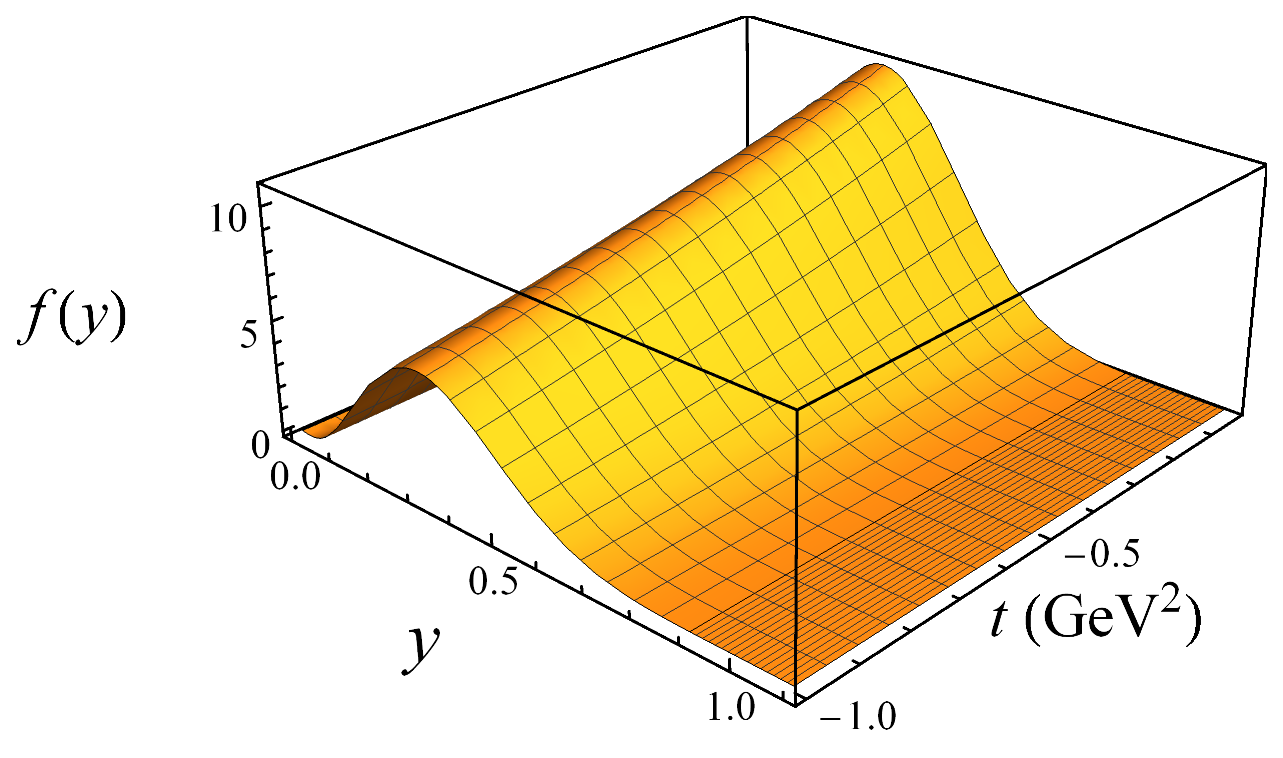
\includegraphics[scale=0.5]{pic/b-f-3D}

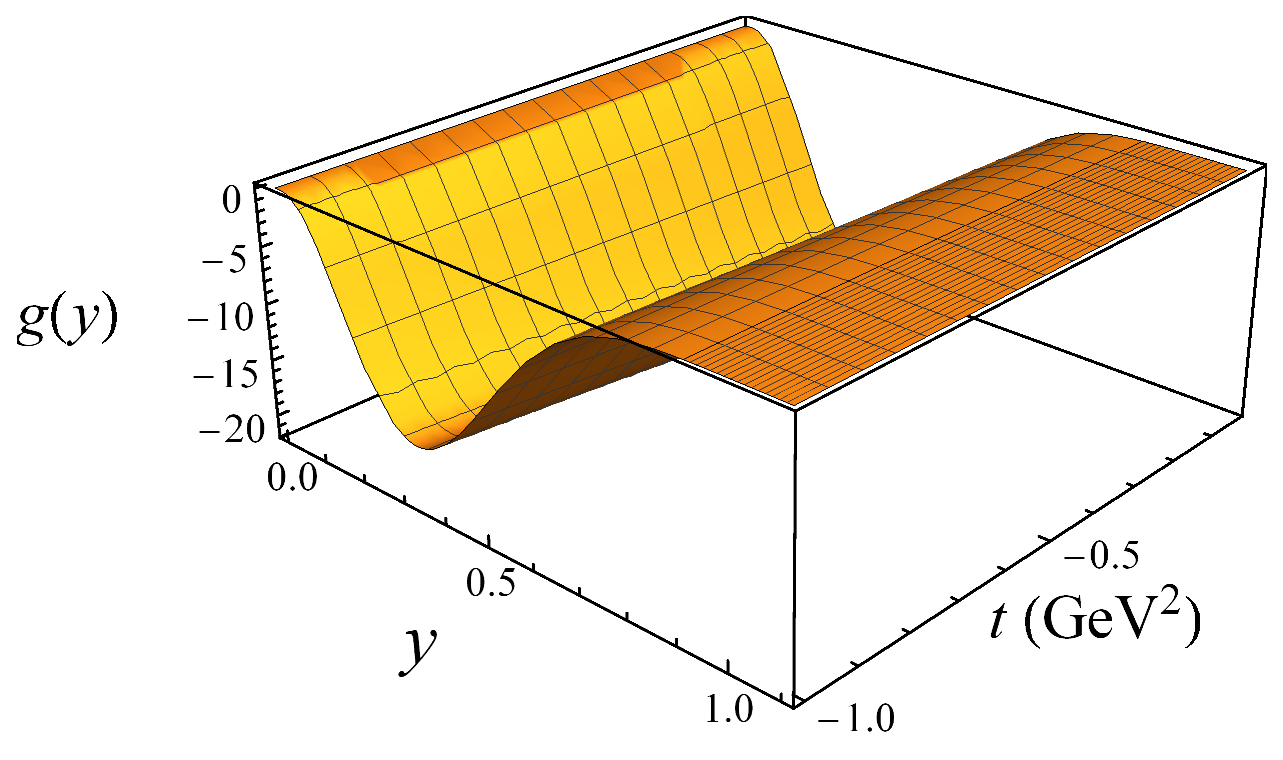
\includegraphics[scale=0.5]{pic/b-g-3D}

\caption{3 dimension picture from diagram b}

\end{figure}


\subsection{diagram c}

For diagram c in fig.1, the equation is similar to diagram b which
is
\[
\Gamma_{c}^{+}=\int\cancel{k}\gamma_{5}\widetilde{F}^{2}(k)\frac{1}{D_{\phi}(k)}\frac{\cancel{p'}-\cancel{k}+m_{N}}{D_{B}(p'-k)}\frac{i\sigma^{+\nu}q_{\nu}}{2M_{N}}\frac{\cancel{p}-\cancel{k}+m_{N}}{D_{B}(p-k)}\cancel{k}\gamma_{5}\delta(y+\xi-\frac{k^{+}}{P^{+}})
\]

And the result of splitting function is also similar to diagram b.
The splitting function can be expressed as 
\begin{align*}
f & =f_{res}+\delta f\\
g & =g_{res}+\delta g
\end{align*}

the $f_{res}$ and $g_{res}$ is the normal integral part and the
second term is the $\delta$ function. First, the $\xi$ independece
is checked. 
\begin{align*}
\int_{-\xi}^{1}dyf & =-1.86186\\
\int_{-\xi}^{1}dyg & =-2.15724
\end{align*}

The $\delta g=-5.2702\delta(y+\xi)$, but the $\delta f$ changes
with different $\xi$ that is
\begin{align*}
\delta f & =-0.106469\delta(y+\xi),\xi=0.1\\
\delta f & =-0.439183\delta(y+\xi),\xi=0.2
\end{align*}

The normal integral part of splitting function is similar to the diagram
b condition. When $\xi=0.1,Q^{2}=1GeV^{2}$, the splitting function
looks like this 

\begin{figure}
\includegraphics{pic/c-f1}

\caption{$f_{1}$from diagram c}
\end{figure}

\begin{figure}
\includegraphics{pic/c-f2}

\caption{$f_{2}$from diagram c}
\end{figure}

\begin{figure}
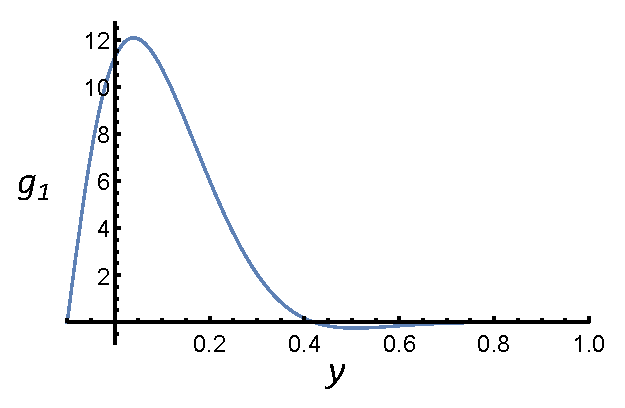
\includegraphics{pic/c-g1}

\caption{$g_{1}$from diagram c}
\end{figure}

\begin{figure}
\includegraphics{pic/c-g2}

\caption{$g_{2}$from diagram c}
\end{figure}

Also the splitting function is not a $\delta$ function when $\xi$
goes to 0. Just like diagram b, we get 
\begin{figure}
\includegraphics[scale=0.5]{pic/c-f-xi1} \includegraphics[scale=0.5]{pic/c-f-xi2}

\includegraphics[scale=0.5]{pic/c-f-xi3}

\caption{$f$ when $\xi=0.01,0.001,0.0001$}
\end{figure}
\begin{figure}
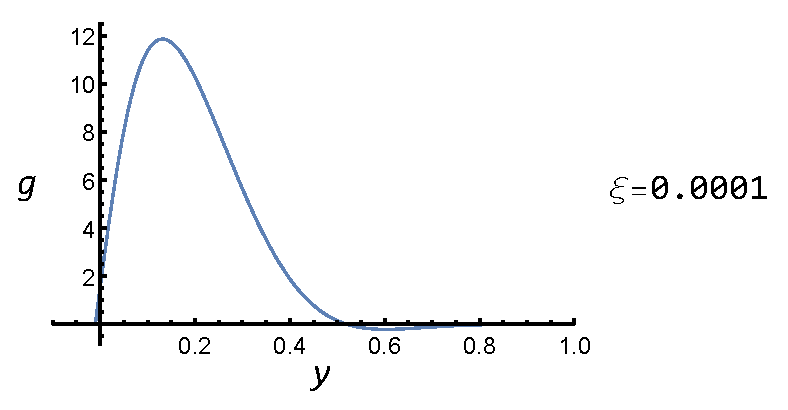
\includegraphics[scale=0.5]{pic/c-g-xi1} \includegraphics[scale=0.5]{pic/c-g-xi2}

\includegraphics[scale=0.5]{pic/c-g-xi3}

\caption{$g$ when $\xi=0.01,0.001,0.0001$}
\end{figure}

\begin{figure}
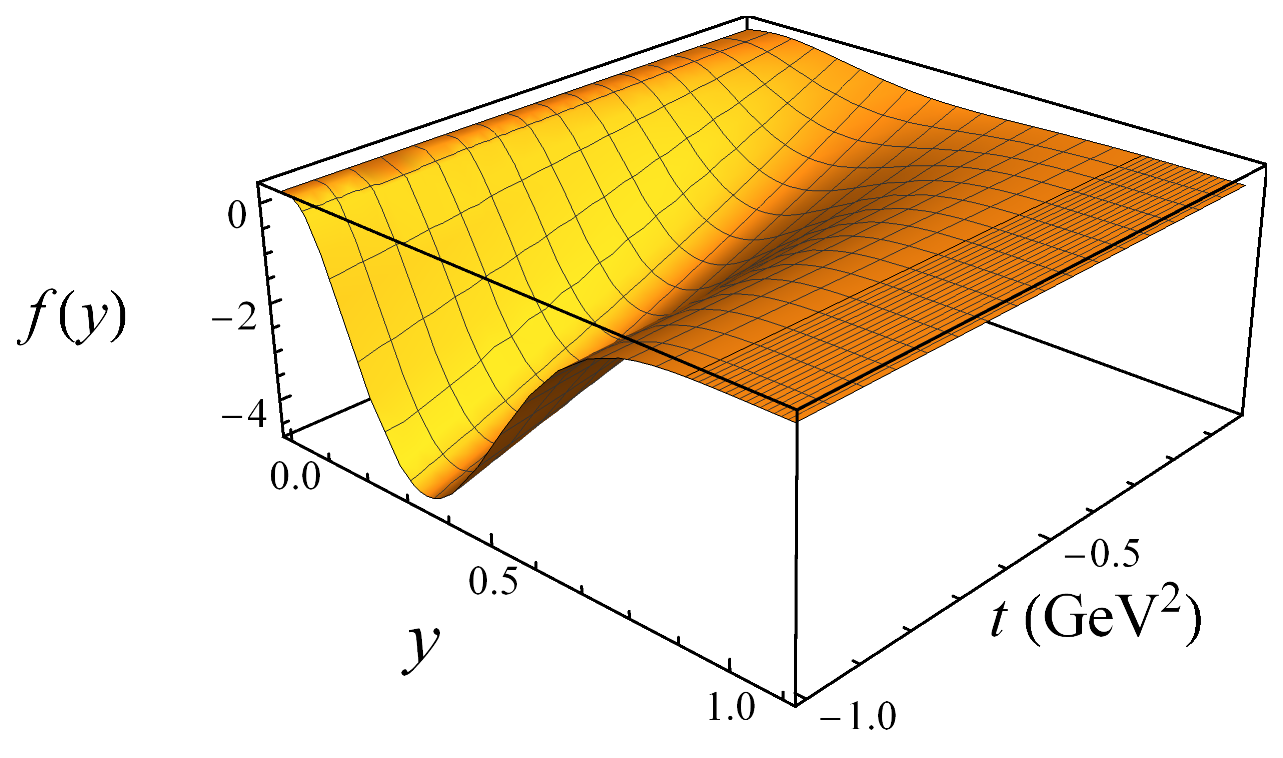
\includegraphics[scale=0.5]{pic/c-f-3D}

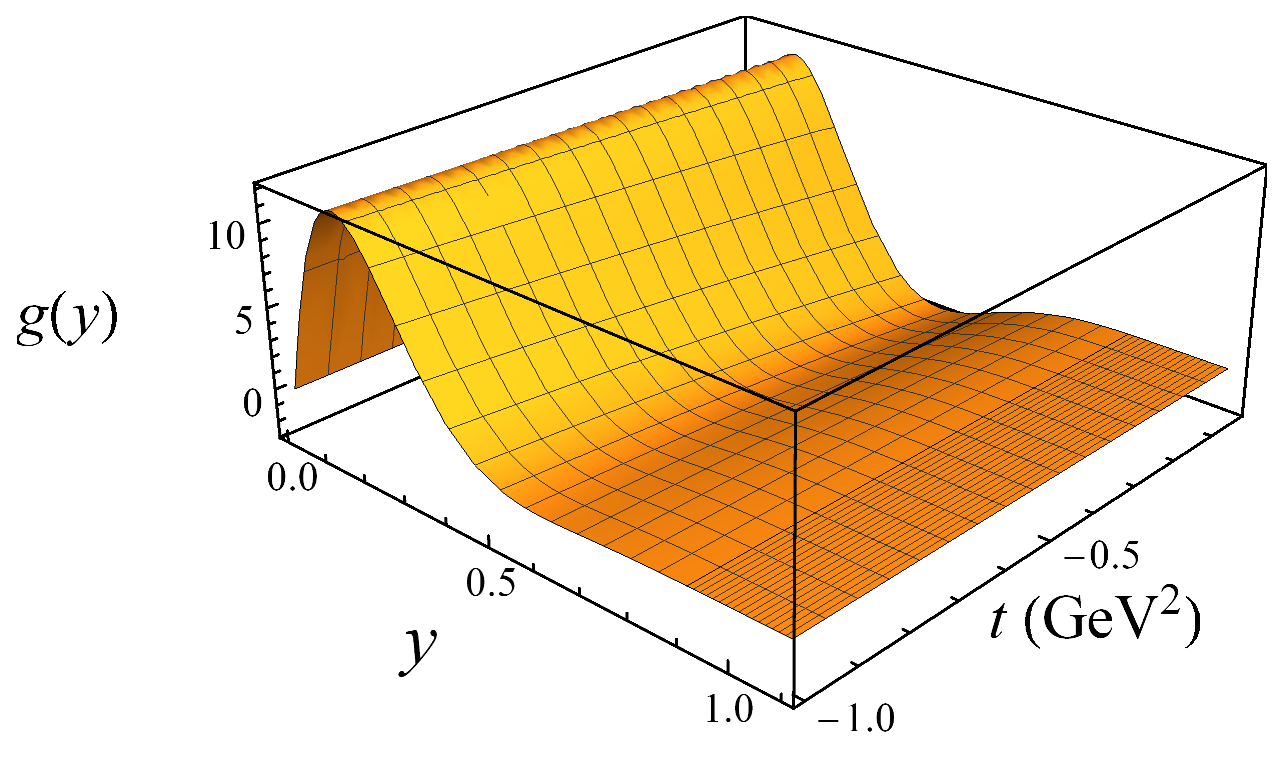
\includegraphics[scale=0.5]{pic/c-g-3D}

\caption{3 dimension picture from diagram c}
\end{figure}


\section{diagram d and e (normal KR)}

For diagram d and e, the KR diagram with normal vertex. The calculation
is finished and the result is checked by compare the integral with
the form factor result. The contribution from these diagrams is 
\[
\Gamma_{(d+e)}^{+}=\int F(k)^{2}\frac{i}{D_{\phi}(k)}(\cancel{k}\gamma_{5}\frac{\cancel{p'}-\cancel{k}+M_{B}}{D_{B}(p'-k)}\gamma^{\mu}\gamma_{5}+\gamma^{\mu}\gamma_{5}\frac{\cancel{p}-\cancel{k}+M_{B}}{D_{B}(p-k)}\cancel{k}\gamma_{5})\delta(y-\frac{k^{+}}{P^{+}})
\]

The result is separated into two part
\begin{align*}
f & =f_{res}+\delta f\\
g & =g_{res}+\delta g
\end{align*}

The lowest moment of splitting function should be equal to the form
factor calculation 
\begin{align*}
F(q)*\int dy(f_{res}+\delta f) & =F_{1}\\
F(q)*\int dy(g_{res}+\delta g) & =F_{2}
\end{align*}

And when $Q^{2}=1MeV^{2}$ the integral is 
\begin{align*}
\int dy(f_{res}+\delta f) & =0.0696379\\
F_{1} & =0.0174106\\
F(q) & =\frac{1}{4}
\end{align*}

The $g$ part should be 0, but the result from splitting function
is not very small, $\int dy(g_{res}+\delta g)=-0.000376259$. We can
exam the function $g(y)$, the image can be given as

\begin{figure}
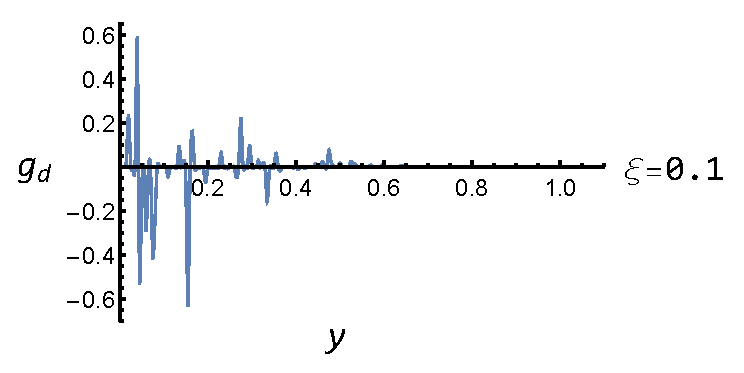
\includegraphics{pic/d-g-xi1}

\caption{$g(y)$ from diagram d}
\end{figure}

First, we can choose more point when we fit the function and calculate
the integral with higher precision. Then at most points, the function
is smaller than $10^{-6}$. The image now become.
\begin{figure}
\includegraphics{pic/d-g-xi1-hp}

\caption{$g(y)$ from diagram d with higher precison}

\end{figure}

For the points where the value is still around $0.01$, one can separate
the range of $k^{\perp}$, from $[0,\infty]$ to $[0,10]+[10,\infty]$.
The $g(y)$ will become around $10^{-8}$. So the $g(y)$ is 0 in
these two diagram. 

The $\delta f=5.270055544$

The normal part of $f$ with $\xi=0.1$ can be given as 
\begin{figure}
\includegraphics[scale=0.5]{pic/d-f-xi1}\includegraphics[scale=0.5]{pic/e-f-xi1}

\caption{$f_{res}$ from diagram d and e}
\end{figure}
 

The images show that the two diagrams have same contribution to the
form factor, but different contribution to the splitting function
although the difference is not significant when $\xi=0.1$.

When $\xi$ goes to 0, the splitting function behave like 
\begin{figure}
\includegraphics[scale=0.5]{pic/d-f-xi01}\includegraphics[scale=0.5]{pic/d-f-xi001}

\includegraphics[scale=0.5]{pic/d-f-xi0001}

\caption{$f$ from diagram d with small $\xi$}

\end{figure}

\begin{figure}
\includegraphics[scale=0.5]{pic/e-f-xi01}\includegraphics[scale=0.5]{pic/e-f-xi001}

\includegraphics[scale=0.5]{pic/e-f-xi0001}

\caption{$f$ from diagram e with small $\xi$}
\end{figure}

\begin{figure}
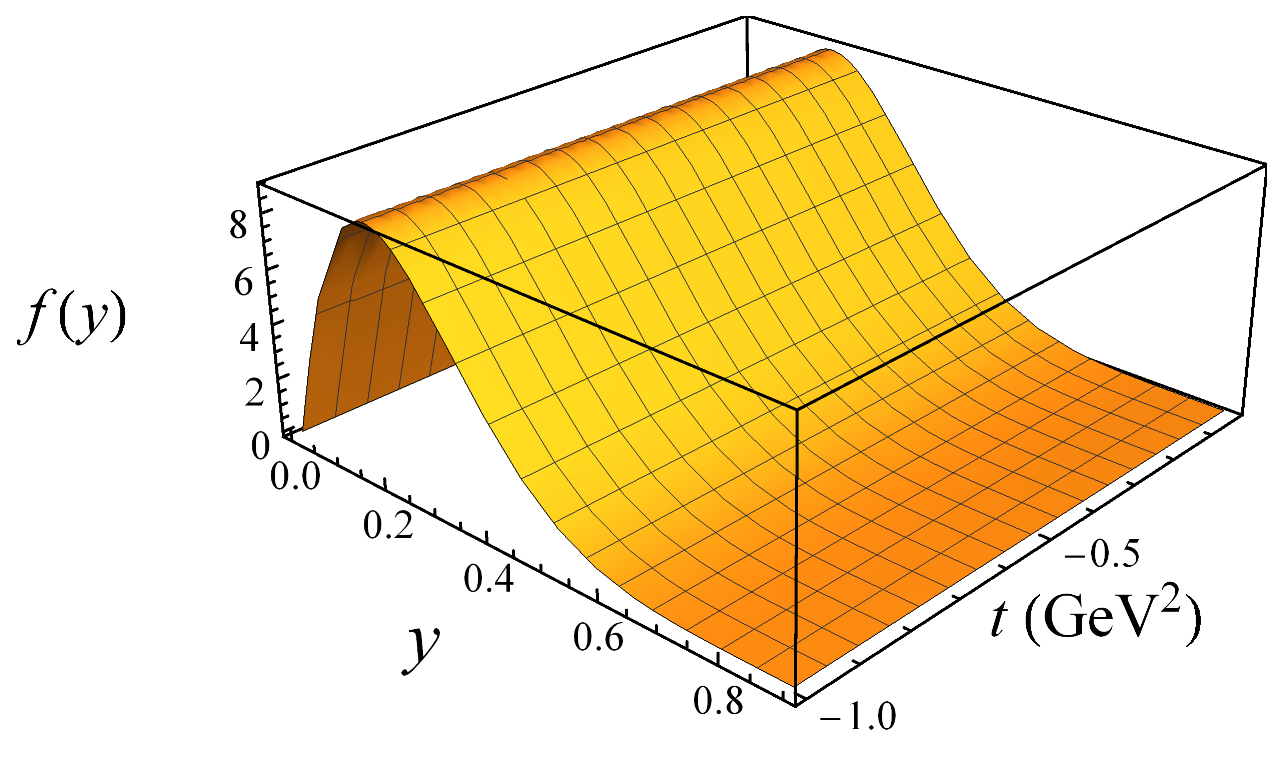
\includegraphics[scale=0.5]{pic/d-f-3D}

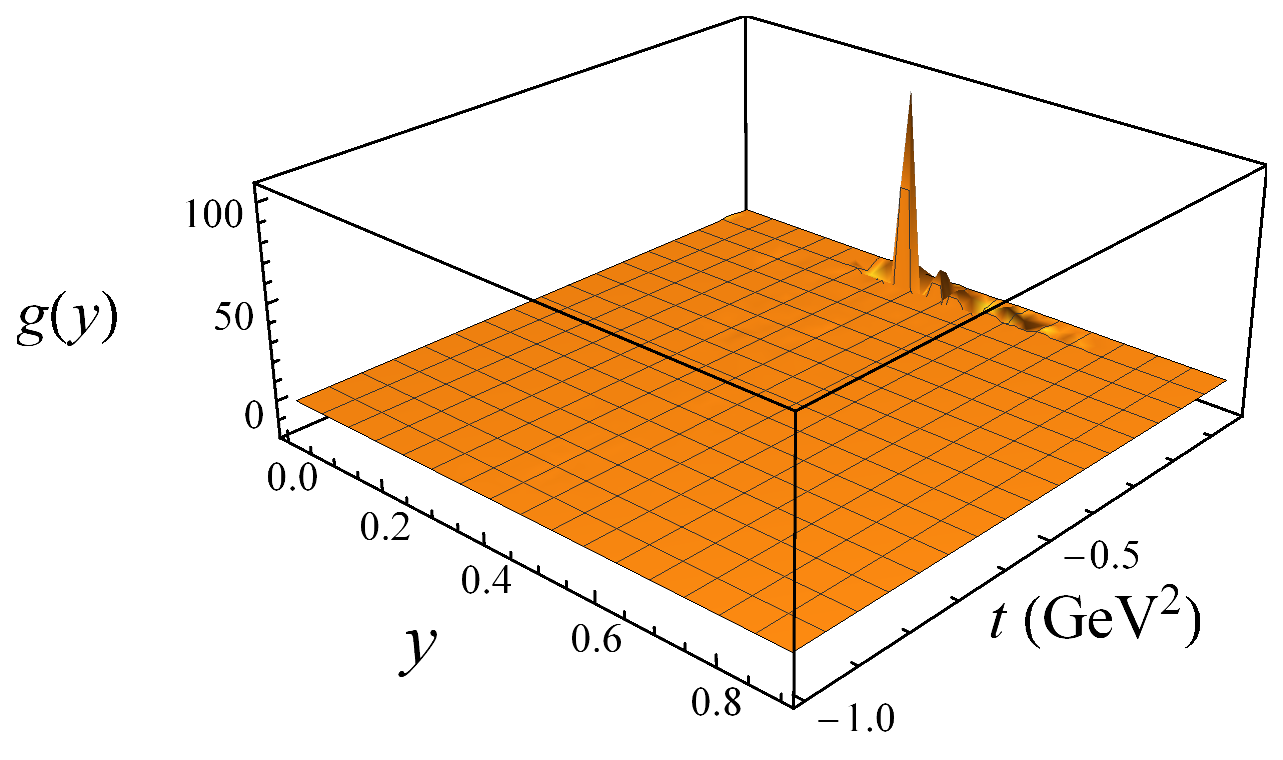
\includegraphics[scale=0.5]{pic/d-g-3D}

\caption{3 dimension picture from diagram d}
\end{figure}

\begin{figure}
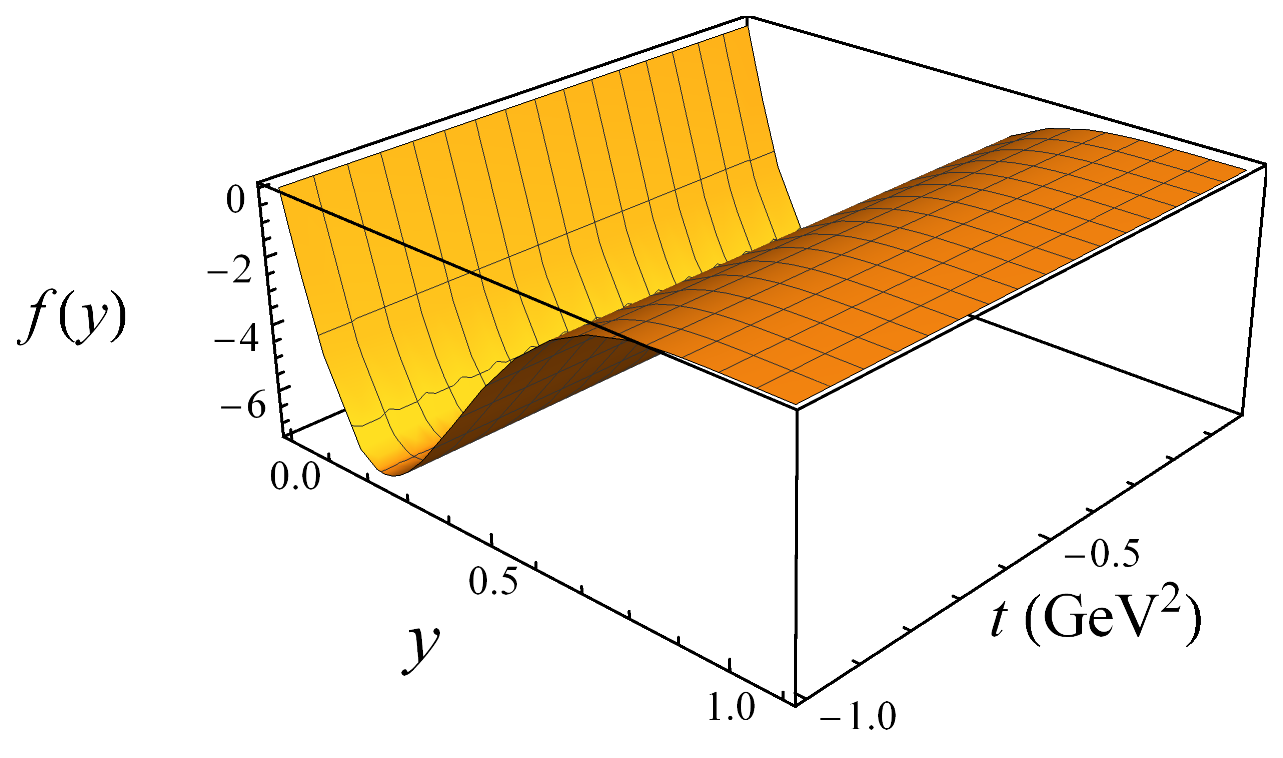
\includegraphics[scale=0.5]{pic/e-f-3D}

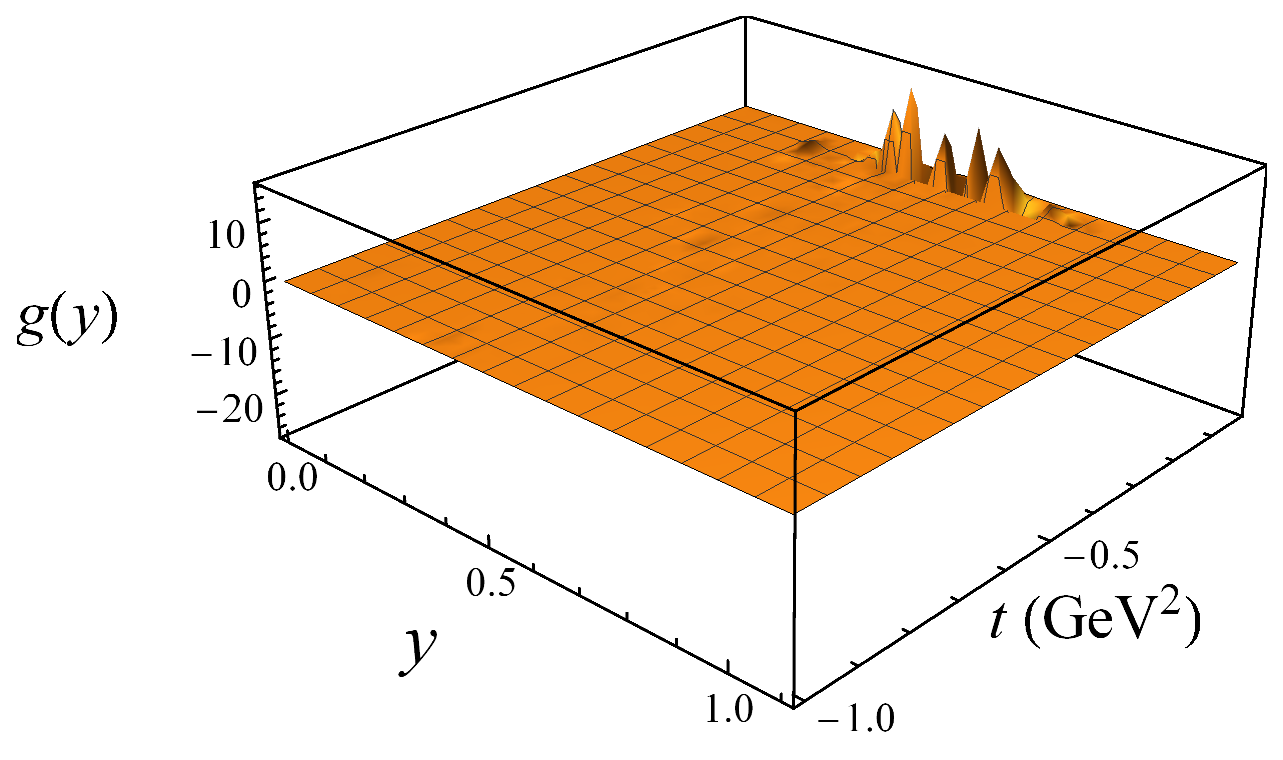
\includegraphics[scale=0.5]{pic/e-g-3D}

\caption{3 dimension picture from diagram e}
\end{figure}

The splitting function has normal part when $\xi=0$ like diagram
b.

\section{diagram f and g (additional KR)}

For diagram f and g, the additional KR diagram from nonlocal Lagrangian.
The contribution can be expressed as
\begin{align*}
\Gamma_{(f+g)}^{+} & =\int\frac{d^{4}k}{(2\pi)^{4}}\frac{i}{D_{\phi}(k)}\tilde{F}(k)[\frac{2k^{+}-q^{+}}{2kq-q^{2}}(\tilde{F}(k)-\tilde{F}(k-q))\cancel{k}\gamma_{5}\frac{\cancel{p'}-\cancel{k}+M_{B}}{D_{B}(p'-k)}(\cancel{k}-\cancel{q})\gamma_{5}\\
 & +\frac{2k^{+}+q^{+}}{2kq+q^{2}}(\tilde{F}(k+q)-\tilde{F}(k))(\cancel{k}+\cancel{q})\gamma_{5}\frac{\cancel{p}-\cancel{k}+M_{B}}{D_{B}(p-k)}\cancel{k}\gamma_{5}]\delta(y-\frac{k^{+}}{P^{+}})
\end{align*}
The splitting function still is separated to two part. 
\begin{align*}
f & =f_{res}+\delta f\\
g & =g_{res}+\delta g
\end{align*}

These two diagrams have same $\delta$ term 
\begin{align*}
\delta f & =-2.6351\delta(y)\\
\delta g & =0
\end{align*}

The normal integral is different from other cases. The lowest moment
of splitting function from single diagram is $\xi$ dependent and
two result are different. In the normal KR diagram, the result is
same no matter the position of the vertex. The lowest moment of the
normal part splitting function from diagram f is listed below with
$\xi=0.1\ Q^{2}=1GeV^{2}$ ignoring some coefficient
\begin{align*}
\int dyf_{f} & =3.614491865\;\xi=0.1\\
\int dyf_{f} & =4.121612607\;\xi=0.2
\end{align*}

And for diagram g the result is 
\begin{align*}
\int dyf_{g} & =2.600249573\;\xi=0.1\\
\int dyf_{g} & =2.093126056\;\xi=0.2
\end{align*}

The result of these two diagram is
\begin{align*}
\int dyf & =\int dy(f_{f}+f_{g})\\
 & =6.21474\;\xi=0.1\\
 & =6.21474\;\xi=0.2
\end{align*}

For $g$ part, the result is same.
\begin{align*}
\int dyg_{f} & =1.890929104\;\xi=0.1\\
\int dyg_{f} & =1.383799830\;\xi=0.2
\end{align*}
\begin{align*}
\int dyg_{g} & =2.905187580\;\xi=0.1\\
\int dyg_{g} & =3.412314403\;\xi=0.2
\end{align*}

\begin{align*}
\int dyg & =\int dy(g_{f}+g_{g})\\
 & =4.79612\;\xi=0.1\\
 & =4.79611\;\xi=0.2
\end{align*}

And compared with the form factor result, we should have
\begin{align*}
\tilde{F}(q)\int dyf & =F_{1}\\
\tilde{F}(q)\int dyg & =F_{2}
\end{align*}

In the other diagram like diagram d and e, the normal KR diagrams,
the equation is satisfied even if only one diagram's contribution
considered. But for diagram f and g, the additional KR diagrams, we
must consider two diagram's contribution together. With $\xi=0.1\ Q^{2}=1GeV^{2}$,
the form factor should be
\begin{align*}
\tilde{F}(q)\int dyf & =0.00695274\\
\tilde{F}(q)\int dyg & =0.0353042
\end{align*}

While the form factor result from previous work is
\begin{align*}
F_{1} & =0.00695275\\
F_{2} & =0.0353042
\end{align*}

The image of the splitting function is given below.
\begin{figure}
\includegraphics[scale=0.5]{pic/f-f-xi1}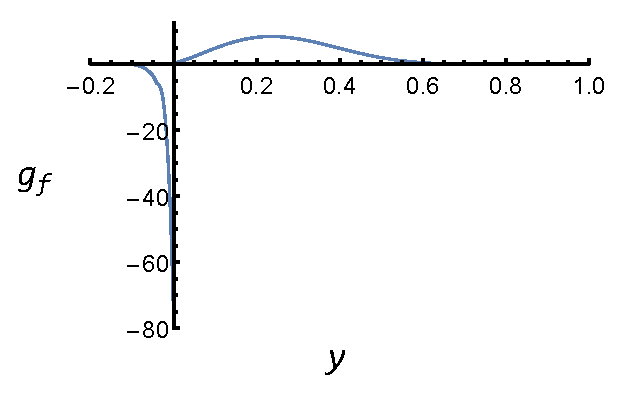
\includegraphics[scale=0.5]{pic/f-g-xi1}

\caption{$f$ and $g$ from diagram f}
\end{figure}

\begin{figure}
\includegraphics[scale=0.5]{pic/g-f-xi1}\includegraphics[scale=0.5]{pic/g-g-xi1}

\caption{$f$ and $g$ from diagram g}
\end{figure}

\begin{figure}
\includegraphics[scale=0.5]{pic/f+g-f-xi1}\includegraphics[scale=0.5]{pic/f+g-g-xi1}

\caption{$f$ and $g$ from diagram f+g}
\end{figure}

Where $f_{f+g}=f_{f}+f_{g}\;g_{f+g}=g_{f}+g_{g}$

When $\xi$ goes to 0, the splitting function act like images showed
below.
\begin{figure}
\includegraphics[scale=0.5]{pic/f-f-xix1}\includegraphics[scale=0.5]{pic/f-f-xix2}

\includegraphics[scale=0.5]{pic/f-f-xix3}

\caption{$f$ from diagram f with small $\xi$}
\end{figure}

\begin{figure}
\includegraphics[scale=0.5]{pic/f-g-xix1}\includegraphics[scale=0.5]{pic/f-g-xix2}

\includegraphics[scale=0.5]{pic/f-g-xix3}

\caption{$g$ from diagram f with small $\xi$}
\end{figure}

\begin{figure}
\includegraphics[scale=0.5]{pic/g-f-xix1}\includegraphics[scale=0.5]{pic/g-f-xix2}

\includegraphics[scale=0.5]{pic/g-f-xix3}

\caption{$f$ from diagram g with small $\xi$}
\end{figure}

\begin{figure}
\includegraphics[scale=0.5]{pic/g-g-xix1}\includegraphics[scale=0.5]{pic/g-g-xix2}

\includegraphics[scale=0.5]{pic/g-g-xix3}

\caption{$g$ from diagram g with small $\xi$}
\end{figure}

\begin{figure}
\includegraphics[scale=0.5]{pic/f-f-3D}

\includegraphics[scale=0.5]{pic/f-g-3D}

\caption{3 dimension picture from diagram f}
\end{figure}
\begin{figure}
\includegraphics[scale=0.5]{pic/g-f-3D}

\includegraphics[scale=0.5]{pic/g-g-3D}

\caption{3 dimension picture from diagram g}
\end{figure}

The $f$ function from both two diagrams become $\delta$ function
when $\xi$ is 0, and the $g$ function are goes to a certain function.

Next, the 3 dimension images of splitting functions from some of the
Feynman diagrams have been obtained. With $\xi=0.1$, the splitting
function $f(y,\xi,t)$ or $g(y,\xi,t)$ are showed above.

\part{Decuplet}

\section{diagram n and o (rainbow)}

For diagram n, the decuplet rainbow diagram, the contribution is 
\[
\Gamma_{n}^{+}=\int\frac{d^{4}k}{(2\pi)^{4}}k_{\lambda}\Theta^{\lambda\sigma}\tilde{F}(k)\frac{1}{D_{\phi}(k)}\frac{\cancel{p'}-\cancel{k}+M_{B}}{D_{B}(p'-k)}S_{\sigma\alpha}(p'-k)\gamma^{\alpha\beta+}\frac{\cancel{p}-\cancel{k}+M_{B}}{D_{B}(p-k)}S_{\beta\rho}(p-k)\Theta^{\rho\nu}k_{\nu}\tilde{F}(k)\delta(y-\frac{k^{+}}{P^{+}})
\]

Same as octet condition, we need to get the $\delta$ term. However
now the $\Gamma_{n}^{+}$ is this form
\[
\Gamma_{n}^{+}=\int\frac{d^{4}k}{(2\pi)^{4}}\frac{k^{-4}+k^{-3}+k^{-2}+k^{-}+c}{D_{\phi}D_{\Lambda}^{4}D_{B}D'_{B}}
\]

so the $\delta$ term we separated will look like this form 
\[
\int\frac{d^{4}k}{(2\pi)^{4}}\frac{k^{-2}+k^{-}+c}{D_{\phi}(k)D_{\Lambda}^{4}(k)}
\]

while in octet condition, the $\delta$ term is like $\frac{c}{D_{\phi}(k)D_{\Lambda}^{4}(k)}$.The
$\int d^{4}k\frac{1}{D_{\phi}^{a}(k)D_{\Lambda}^{b}(k)}$ is obtained
by this method
\begin{align*}
\int dk^{-}\frac{1}{D_{\phi}^{a}(k)D_{\Lambda}^{b}(k)} & =\frac{\Gamma(a+b)}{\Gamma(a)\Gamma(b)}\int dk^{-}\int_{0}^{1}dx\frac{x^{a-1}(1-x)^{b-1}}{(xD_{\phi}+(1-x)D_{\Lambda})^{a+b}}\\
 & =\frac{\Gamma(a+b)}{\Gamma(a)\Gamma(b)}\int dk^{-}\int_{0}^{1}dx\frac{x^{a-1}(1-x)^{b-1}}{(k^{2}-\Omega)^{a+b}}\\
 & =\frac{2\pi i\Gamma(a+b)}{(a+b-1)!\Gamma(a)\Gamma(b)}\int dk^{-}\int_{0}^{1}dx\frac{\partial^{a+b-2}}{\partial\Omega^{a+b-2}}\frac{x^{a-1}(1-x)^{b-1}}{(k^{2}-\Omega)^{2}}
\end{align*}

where $\Omega=xm_{\phi}^{2}+(1-x)\Lambda^{2}$. 

So in same way, $\int d^{4}k\frac{k^{-n}}{D_{\phi}^{a}(k)D_{\Lambda}^{b}(k)}$
is 
\[
\int dk^{-}\frac{k^{-n}}{D_{\phi}^{a}(k)D_{\Lambda}^{b}(k)}=\frac{\Gamma(a+b)}{\Gamma(a)\Gamma(b)}\int dk^{-}\int_{0}^{1}dxx^{a-1}(1-x)^{b-1}\frac{k^{-n}}{(k^{2}-\Omega)^{a+b}}
\]

This term $\int dk^{-}\frac{k^{-n}}{(k^{2}-\Omega)^{a+b}}$ can be
changed to 
\[
\int dk^{-}\frac{k^{-n}}{(k^{2}-\Omega)^{a+b}}\rightarrow\int dk^{-}\frac{\partial^{n}}{\partial k^{+n}}\frac{1}{(k^{2}-\Omega+i\epsilon)^{a+b-n}}
\]

Then the whole term will be 
\begin{align*}
\int dk^{-}\frac{k^{-n}}{D_{\phi}^{a}(k)D_{\Lambda}^{b}(k)} & \rightarrow\int dk^{+}\frac{\partial^{n}}{\partial k^{+n}}\frac{\Gamma(a+b)}{\Gamma(a)\Gamma(b)}\int_{0}^{1}dxx^{a-1}(1-x)^{b-1}\frac{\partial^{a+b-2-n}}{\partial\Omega^{a+b-2-n}}\int dk^{-}\frac{1}{(k^{2}-\Omega)^{2}}\\
 & \rightarrow\int dk^{+}\frac{\partial^{n}}{\partial k^{+n}}\delta(k^{+})
\end{align*}

And we use this approximate value for the derivaton of $\delta$ function
\begin{align*}
\frac{\partial}{\partial k^{+}}\delta(k^{+}) & =\frac{\delta(k^{+})}{k^{+}}\\
\frac{\partial^{2}}{\partial k^{+2}}\delta(k^{+}) & =0
\end{align*}

So the $\delta$ term calculated in this way has form like this
\begin{align*}
\delta term & =\int\frac{d^{4}k}{(2\pi)^{4}}\frac{k^{-2}+k^{-}+c}{D_{\phi}(k)D_{\Lambda}^{4}(k)}\\
 & =A\frac{1}{y}\delta(y)+B\delta(y)
\end{align*}

The result of this diagram is, which is $\xi$ independent 
\begin{align*}
\int dyf(y) & =2.9731\\
\int dyg(y) & =-3.3845
\end{align*}

\begin{figure}
\includegraphics[scale=0.5]{pic/n-f1-0\lyxdot 1}\includegraphics[scale=0.5]{pic/n-g1-0\lyxdot 1}

\caption{$f$ and $g$ from diagram n}
\end{figure}


\subsection{diagram o}

For diagram o in Fig.1, the decuplet rainbow diagram with magnetic
vertex, the contribution is 
\[
\Gamma_{o}^{+}=\int\frac{d^{4}k}{(2\pi)^{4}}k_{\lambda}\Theta^{\lambda\sigma}\tilde{F}(k)\frac{1}{D_{\phi}(k)}\frac{\cancel{p'}-\cancel{k}+M_{B}}{D_{B}(p'-k)}S_{\sigma\alpha}(p'-k)\frac{\sigma^{+\beta}q_{\beta}}{2M_{B}}\frac{\cancel{p}-\cancel{k}+M_{B}}{D_{B}(p-k)}S_{\alpha\rho}(p-k)\Theta^{\rho\nu}k_{\nu}\tilde{F}(k)\delta(y-\frac{k^{+}}{P^{+}})
\]

The $\delta$ term for diagram o has this form,
\[
\delta term=\int\frac{d^{4}k}{(2\pi)^{4}}\frac{k^{-3}+k^{-2}+k^{-}+c}{D_{\phi}(k)D_{\Lambda}^{4}(k)}
\]

The detail of this diagram's calculation has been showed in other
notes. There were several problems in the first version of the calculation
which were solved quickly. The problem which bothered me so long is
that in A part I forget to check the $k^{+}$ part.

Now we can get a $\xi$ independent result which agrees with the form
factor result.
\begin{align*}
\int dyf(y) & =-0.003946\\
\int dyg(y) & =4.3472
\end{align*}

The pictures of the normal part splitting function are showed below,.

\begin{figure}
\includegraphics[scale=0.5]{pic/o-f1-0\lyxdot 1}\includegraphics[scale=0.5]{pic/o-g1-0\lyxdot 1}

\caption{$f$ and $g$ from diagram o}
\end{figure}


\section{diagram p and q (transition)}

For diagram p and diagram q, the rainbow diagram with a octet decuplet
transition vertex, the contribution is 
\begin{align*}
\Gamma_{p+q}^{+} & =\int\frac{d^{4}k}{(2\pi)^{4}}\frac{\tilde{F^{2}}(k)}{D_{\phi}(k)}[-\cancel{k}\gamma_{5}\frac{\cancel{p'}-\cancel{k}+M_{B}}{D_{B}(p'-k)}\cancel{q}\gamma_{5}\frac{\cancel{p}-\cancel{k}+M'_{B}}{D'_{B}(p-k)}S^{+\rho}(p-k)\Theta^{\rho\nu}k_{\nu}\\
 & +\cancel{k}\gamma_{5}\frac{\cancel{p'}-\cancel{k}+M_{B}}{D_{B}(p'-k)}\gamma^{+}\gamma_{5}q^{\lambda}\frac{\cancel{p}-\cancel{k}+M'_{B}}{D'_{B}(p-k)}S_{\lambda\rho}(p-k)\Theta^{\rho\nu}k_{\nu}\\
 & -k_{\lambda}\Theta^{\lambda\nu}\frac{\cancel{p'}-\cancel{k}+M'_{B}}{D'_{B}(p'-k)}S_{\nu\rho}(p'-k)q^{\rho}\gamma^{+}\gamma_{5}\frac{\cancel{p}-\cancel{k}+M_{B}}{D_{B}(p-k)}\cancel{k}\gamma_{5}\\
 & +k_{\lambda}\Theta^{\lambda\nu}\frac{\cancel{p'}-\cancel{k}+M'_{B}}{D'_{B}(p'-k)}S_{\nu}^{+}(p'-k)\cancel{q}\gamma_{5}\frac{\cancel{p}-\cancel{k}+M_{B}}{D_{B}(p-k)}\cancel{k}\gamma_{5}]\delta(y-\frac{k^{+}}{P^{+}})
\end{align*}

The $\delta$ term for diagram p and q has this form,
\[
\delta term=\int\frac{d^{4}k}{(2\pi)^{4}}\frac{k^{-2}+k^{-}+c}{D_{\phi}(k)D_{\Lambda}^{4}(k)}
\]

where the propagator with prime is the decuplet baryon propagator
and without prime is a octet baryon propagator.

The $\xi$ independent first moment of these two diagrams is
\begin{align*}
\int dyf(y) & =-1.1088\\
\int dyg(y) & =-6.0569
\end{align*}

\begin{figure}
\includegraphics[scale=0.5]{pic/p-f-0\lyxdot 1}\includegraphics[scale=0.5]{pic/p-g-0\lyxdot 1}

\caption{$f$ and $g$ from diagram p}
\end{figure}

\begin{figure}
\includegraphics[scale=0.5]{pic/q-f-0\lyxdot 1}\includegraphics[scale=0.5]{pic/q-g-0\lyxdot 1}

\caption{$f$ and $g$ from diagram q}
\end{figure}


\section{diagram r and s (normal KR)}

For diagram r and diagram s, the KR diagram, the contribution is 
\[
\Gamma_{r+s}^{+}=\int\frac{d^{4}k}{(2\pi)^{4}}\frac{\tilde{F^{2}}(k)}{D_{\phi}(k)}[k_{\nu}\Theta^{\nu\sigma}\frac{\cancel{p'}-\cancel{k}+M_{B}}{D_{B}(p-k)}S_{\sigma\rho}(p'-k)\Theta^{\rho+}+\Theta^{+\sigma}\frac{\cancel{p}-\cancel{k}+M_{B}}{D_{B}(p-k)}S_{\sigma\rho}(p-k)\Theta^{\rho\nu}k_{\nu}]\delta(y-\frac{k^{+}}{P^{+}})
\]

The $\delta$ term for diagram r and s has this form,
\[
\delta term=\int\frac{d^{4}k}{(2\pi)^{4}}\frac{k^{-}+c}{D_{\phi}(k)D_{\Lambda}^{4}(k)}
\]

The KR diagram with decuplet intermediate is similar to the addition
KR diagram with octet intermediate. For single diagram, the first
moment is not $\xi$ independent but the sum of two diagram is $\xi$
independent. For example, for diagram r
\begin{align*}
\int dyf_{r}(y) & =0.8812\ \xi=0.1\\
\int dyf_{r}(y) & =0.7456\ \xi=0.2\\
\int dyg_{r}(y) & =-1.2202\ \xi=0.1\\
\int dyg_{r}(y) & =-1.0846\ \xi=0.2
\end{align*}

And for diagram s 
\begin{align*}
\int dyf_{s}(y) & =1.1524\ \xi=0.1\\
\int dyf_{s}(y) & =1.2880\ \xi=0.2\\
\int dyg_{s}(y) & =-1.4914\ \xi=0.1\\
\int dyg_{s}(y) & =-1.0846\ \xi=0.2
\end{align*}

The sum is
\begin{align*}
\int dyf & =2.0337\\
\int dyg & =-2.7116
\end{align*}

which is agreed with the form factor calculation. When the external
partical is proton and the meson is $\pi^{+}$, the form factor is
with $Q=1$
\begin{align*}
F_{1} & =0.00726205\\
F_{2} & =-0.00968274
\end{align*}

The coefficient I dropped in splitting function is $\frac{C_{T\phi}^{2}}{f^{2}}\frac{1}{2(2\pi)^{4}}$,
so the form factor from splitting function is 
\begin{align*}
F_{1} & =\tilde{F}(q)0.0290478\\
F_{2} & =\tilde{F}(q)(-0.0387304)
\end{align*}

with $\tilde{F}(1)=\frac{1}{4}$
\begin{figure}
\includegraphics[scale=0.5]{pic/r-f-0\lyxdot 1}\includegraphics[scale=0.5]{pic/r-g-0\lyxdot 1}

\caption{$f$ and $g$ from diagram r}

\end{figure}

\begin{figure}
\includegraphics[scale=0.5]{pic/s-f-0\lyxdot 1}\includegraphics[scale=0.5]{pic/s-g-0\lyxdot 1}

\caption{$f$ and $g$ from diagram s}
\end{figure}


\section{diagram t and u (additional KR)}

For diagram t and u, the KR diagram with addition vertex, the contribution
is 
\begin{align*}
\Gamma_{t+u}^{+} & =\int\frac{d^{4}k}{(2\pi)^{4}}\frac{\tilde{F}(k)}{D_{\phi}(k)}[k_{\nu}\Theta^{\nu\sigma}\frac{\cancel{p}-\cancel{k}+M_{B}}{D_{B}(p'-k)}S_{\sigma\rho}(p'-k)\Theta^{\rho\lambda}(k-q)^{\lambda}\frac{2k^{+}-q^{+}}{2kq-q^{2}}(\tilde{F}(k-q)-\tilde{F}(k))\\
 & +(k+q)_{\nu}\Theta^{\nu\sigma}\frac{2k^{+}+q^{+}}{2kq+q^{2}}(\tilde{F}(k+q)-\tilde{F}(k))\frac{\cancel{p}-\cancel{k}+M_{B}}{D_{B}(p-k)}S_{\sigma\rho}(p-k)\Theta^{\rho\lambda}k_{\lambda}]\delta(y-\frac{k^{+}}{P^{+}})
\end{align*}

The $\delta$ term for diagram t and u has this form, because of the
$D_{\Lambda}(k\pm q)$ in the denominator.
\[
\delta term=\int\frac{d^{4}k}{(2\pi)^{4}}\frac{k^{-}+c}{D_{\phi}(k)D_{\Lambda}^{4}(k)}
\]

Just like octet case, the contribution from these two diagrams is
$\xi$ independent, which is
\begin{align*}
\int dyf & =-0.3947\\
\int dyg & =-5.064
\end{align*}

The result agree with form factor calculation. 

\begin{figure}
\includegraphics[scale=0.5]{pic/t-f-0\lyxdot 1}\includegraphics[scale=0.5]{pic/t-g-0\lyxdot 1}

\caption{$f$ and $g$ from diagram t}
\end{figure}

\begin{figure}
\includegraphics[scale=0.5]{pic/u-f-0\lyxdot 1}\includegraphics[scale=0.5]{pic/u-g-0\lyxdot 1}

\caption{$f$ and $g$ from diagram u}
\end{figure}


\part{Convolution formula}

The next step is getting the GPD using convolution formula. As we
discussed, now the convolution formula is
\begin{align*}
\int_{x}^{1}d(1-y)\frac{1}{1-y}f(y,\xi,t)H_{q}(\frac{x}{1-y},\frac{\xi}{1-y},t),\quad1-y & >x>\xi\\
\int_{\xi}^{1}d(1-y)\frac{1}{1-y}f(y,\xi,t)H_{q}(\frac{x}{1-y},\frac{\xi}{1-y},t),\quad1-y & >\xi>x\\
\int_{-\xi}^{\xi}d(1-y)\frac{1}{2\xi}f(y,\xi,t)\frac{1}{\pi}\frac{\xi}{1-y}\int_{s_{0}}^{\infty}ds\frac{Im\Phi(\frac{\frac{x}{\xi}+1}{2},\frac{\frac{1-y}{\xi}+1}{2},s)}{s-t+i\epsilon}\quad\xi & >\{1-y,|x|\}\\
\int_{-x}^{1}d(1-y)\frac{1}{1-y}f(y,\xi,t)H_{q}(\frac{x}{1-y},\frac{\xi}{1-y},t),\quad- & \xi>x>-1
\end{align*}

where the range of $y$ is $[0,1+\xi]$ and the $1-y\in[-\xi,1]$
which is same with $y$ in meson loop case.

There are two KR additional diagram which ask the range of $y$ to
be $[-2\xi,1-\xi]$ because the residue theory which does not have
result now.

For baryon loop case,the convolution formula is
\begin{align*}
\int_{x}^{1}d(1-y)\frac{1}{1-y}f(y,\xi,t)H_{q}(\frac{x}{1-y},\frac{\xi}{1-y},t),\quad1-y & >x>\xi\\
\int_{\xi}^{1}d(1-y)\frac{1}{1-y}f(y,\xi,t)H_{q}(\frac{x}{1-y},\frac{\xi}{1-y},t),\quad1-y & >\xi>x\\
\int_{-\xi}^{\xi}d(1-y)\frac{1}{2\xi}f(y,\xi,t)\frac{1}{\pi}\frac{\xi}{1-y}\int_{s_{0}}^{\infty}ds\frac{Im\Phi(\frac{\frac{x}{\xi}+1}{2},\frac{\frac{1-y}{\xi}+1}{2},s)}{s-t+i\epsilon}\quad\xi & >\{1-y,|x|\}\\
\int_{-x}^{1}d(1-y)\frac{1}{1-y}f(y,\xi,t)H_{q}(\frac{x}{1-y},\frac{\xi}{1-y},t),\quad- & \xi>x>-1
\end{align*}

and for $E(x,\xi,t)$ the formula is same just replace the $f$ with
$g$.

Then we need the GPD and GDA function of valence quark in proton.
In double distribution representation, the GPDs of proton can be write
in this form\cite{Polyakov}
\begin{align*}
H(x,\xi,t) & =\int_{-1}^{1}d\beta\int_{-1+|\beta|}^{1-|\beta|}d\alpha\delta(x-\beta-\alpha\xi)h(\beta,\alpha,t)\\
E(x,\xi,t) & =\int_{-1}^{1}d\beta\int_{-1+|\beta|}^{1-|\beta|}d\alpha\delta(x-\beta-\alpha\xi)e(\beta,\alpha,t)\\
\tilde{H}(x,\xi,t) & =\int_{-1}^{1}d\beta\int_{-1+|\beta|}^{1-|\beta|}d\alpha\delta(x-\beta-\alpha\xi)\tilde{h}(\beta,\alpha,t)
\end{align*}

which is similar to the meson condition. In fact we do not consider
the D term here because the GPD here is in tree level of proton which
do not have D in second moment.

For $\int d\alpha d\beta\delta(x-\beta-\alpha\xi)h(\beta,\alpha,t)$,
like meson loop case, we have
\begin{align*}
h(\beta,\alpha,t) & =h_{0}(\beta,\alpha)H(\beta,0,t)\\
e(\beta,\alpha,t) & =h_{0}(\beta,\alpha)E(\beta,0,t)\\
\tilde{h}(\beta,\alpha,t) & =h_{0}(\beta,\alpha)\tilde{H}(\beta,0,t)
\end{align*}

where $h_{0}(\beta,\alpha)=\frac{\Gamma(2b+2)}{2^{2b+1}\Gamma^{2}(b+1)}\frac{((1-|\beta|)^{2}-\alpha^{2})^{b}}{(1-|\beta|)^{2b+1}}$. 

The zero skewness GPDs are parameterized as\cite{Diehl2005} 
\begin{align*}
H(x,0,t) & =q(x)exp(tf_{q}(x))\\
E(x,0,t) & =e^{q}(x)exp(tg_{q}(x))\\
\tilde{H}(x,0,t) & =\Delta q(x)exp(tf_{q}(x))
\end{align*}

where the $q,f_{q},e^{q},g_{q}$ is 
\begin{align*}
xq(x) & =A_{0}x^{A_{1}}(1-x)^{A_{2}}e^{A_{3}x}(1+e^{A_{4}}x)^{A_{5}}\\
f_{q}(x) & =\alpha_{1}(1-x)^{3}log\frac{1}{x}+B_{q}(1-x)^{3}+A_{q}x(1-x)^{2}\\
e^{q}(x) & =N_{q}\kappa_{q}x^{-a}(1-x)^{b_{q}}\\
g_{q}(x) & =\alpha_{2}(1-x)^{3}log\frac{1}{x}+D_{q}(1-x)^{3}+C_{q}x(1-x)^{2}
\end{align*}

Here the $f_{q},g_{q}$ is related to the form of $q,e^{q}$, so I
think we need to keep the original result from the reference. 

The GDA does not have a new model. So I follow Fangcheng's method.
And the GDA for proton in DD description is
\begin{align*}
\Phi_{1}(z,\eta,s) & =2(2\eta-1)\int_{-1}^{1}d\beta\int_{-1+|\beta|}^{1-|\beta|}d\alpha\delta(2z-1-(2\eta-1)\beta-\alpha)h_{0}(\beta,\alpha)H(\beta,0,s)\\
\Phi_{2}(z,\eta,s) & =2(2\eta-1)\int_{-1}^{1}d\beta\int_{-1+|\beta|}^{1-|\beta|}d\alpha\delta(2z-1-(2\eta-1)\beta-\alpha)h_{0}(\beta,\alpha)E(\beta,0,s)
\end{align*}

which use the relation between GPD and GDA 
\begin{align*}
1-2z & \leftrightarrow\frac{x}{\xi}\\
1-2\eta & \leftrightarrow\frac{1}{\xi}
\end{align*}

\bibliographystyle{plain}
\nocite{*}
\bibliography{ref/convolution}
 
\end{document}
